\chapter{Prediction Evaluation}\label{prediction_evaluation}
	
	
	\tdic[Prediction is inevitable]{Intro talks about no matter how we do it the data will be spatially incomplete. Prediction is inevitable
		\begin{itemize}
			\item Explain different ones here (can link to background section). Are they any use? Can simple things work?
			\item Extra stuff is beyond the scope of this work
		\end{itemize}
	}
	\tdi{Explain how I will study the performance of the data set}
	\tdi{Present and discuss results}


	Stampfenbachstrasse: (47.386769, 8.539810)
	Schimmelstrasse: (47.370962, 8.523560)

	The remaining part of the project is evaluating whether the implementation would provide useful data or not. As mentioned in section ??\todo{Fill in this reference} a similar project is currently running in Zurich. The \emph{OpenSense}~\cite{opensensezurich} project places sensors on trams and is designed to provide data to the general public with minimal cost. The project uses cheap hardware and accurate stationary measurement stations for calibration. If we look at their maps of information we can see that the readings they provide are only along the tram routes. An example of this, but in Edinburgh, can be seen in figure~\ref{fig:stationarypollutantbuildup}. In order for the data that we would potentially collect, should the project be physically realised, to be useful we would have to be able to accurately predict what the concentrations of chemicals are in areas where we do not have sensor readings. 

	\begin{figure}[H]
	    \begin{center}
	        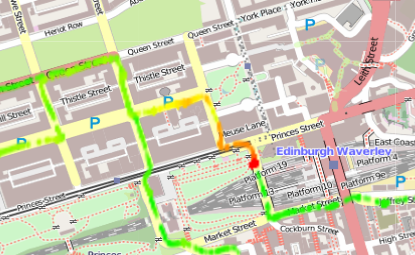
\includegraphics[width=\textwidth]{./images/StationaryPollutantBuildUp.png}
	        \caption{A map of air pollution around Edinburgh city centre. Image uses \emph{Open Street Map}.}
	        \label{fig:stationarypollutantbuildup}
	    \end{center}
	\end{figure}

	If were were to use some statistical method on a dataset similar to that seen in figure~\ref{fig:stationarypollutantbuildup}, we could estimate with some degree of certainty what the pollution levels are in areas where there are no recordings. By doing this we could produce a map similar to the one in figure~\ref{fig:zurichheatmap}.

	\begin{figure}[H]
	    \begin{center}
	        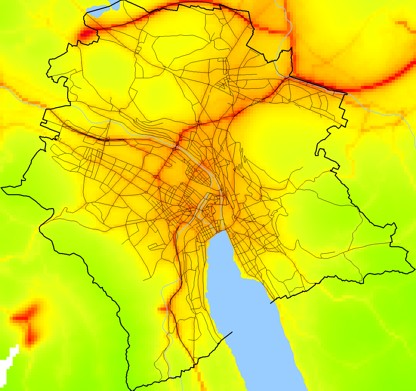
\includegraphics[width=\textwidth]{./images/zurichpm.jpg}
	        \caption{A heatmap of particulate matter in Zurich. The higher pollution levels can clearly be seen to follow transport infrastructure.~\cite{opensensezurich}}
	        \label{fig:zurichheatmap}
	    \end{center}
	\end{figure}

	
	In order to solve this problem and accurately predict the pollution levels, advanced statistical techniques, with a great deal of domain specific information, are required. Doing this would be impractical for the \emph{City of Edinburgh Council}. Instead we will employ existing tools and simpler statistical methods to help us perform this task. By using well known and understood methods, avoiding complex methods such as regression kriging~\cite{regressionkriging}, which are provided in a single tool or package, such as R or Python libraries, we will attempt to prove that this data is at least accurate enough to provide a high level overview of pollution across the city. 

	In order to validate whether our results are correct or not, we will use the freely available data from the OpenSense project and perform our analysis on this. By performing our statistical methods on a dataset from the OpenSense project we will be able to predict the pollution levels at any point in Zurich to within some degree of accuracy. By comparing the values at the same locations as a static measurement station, with the results from said measurement station, we will obtain a metric which informs us of the accuracy of the interpolation method.


